\documentclass[11pt,a4paper]{article}

\usepackage{fontspec}
\usepackage[brazil]{babel}
\usepackage{microtype}
\usepackage[margin=2.3cm]{geometry}
\usepackage{amsmath,amssymb}
\usepackage{graphicx}
\usepackage{booktabs}
\usepackage{tabularx}
\usepackage{array}
\usepackage{xcolor}
\usepackage[most]{tcolorbox}
\usepackage{tikz}
\usetikzlibrary{arrows.meta,positioning,shapes.geometric,fit,calc,decorations.pathreplacing}
\usepackage[american]{circuitikz}
\usepackage{enumitem}
\usepackage{caption}
\usepackage{titlesec}
\usepackage{fancyhdr}
\usepackage{needspace}
\usepackage[hidelinks]{hyperref}

\definecolor{azul}{HTML}{1F5FA8}
\definecolor{verde}{HTML}{2E8B57}
\definecolor{vermelho}{HTML}{D1495B}
\definecolor{amarelo}{HTML}{EDAE49}
\definecolor{cinza}{HTML}{555555}

\titleformat{\section}{\Large\bfseries\color{azul}}{\thesection}{0.8em}{}
\titleformat{\subsection}{\large\bfseries\color{azul!80!black}}{\thesubsection}{0.7em}{}
\titleformat{\subsubsection}{\normalsize\bfseries}{\thesubsubsection}{0.6em}{}

\pagestyle{fancy}
\fancyhf{}
\fancyhead[L]{\small\color{cinza}DAS5109 -- Proposta de Trabalho Final}
\fancyhead[R]{\small\color{cinza}\thepage}
\renewcommand{\headrulewidth}{0.3pt}

\setlist{itemsep=2pt,topsep=4pt}
\setlength{\emergencystretch}{2em}
\captionsetup{font=small,labelfont=bf}

\newtcolorbox{intuicao}[1][]{enhanced,breakable,colback=verde!6,colframe=verde,
  fonttitle=\bfseries,title={Intuição#1},boxrule=0.6pt,arc=2pt,left=6pt,right=6pt}
\newtcolorbox{atencao}[1][]{enhanced,breakable,colback=vermelho!6,colframe=vermelho,
  fonttitle=\bfseries,title={Atenção#1},boxrule=0.6pt,arc=2pt,left=6pt,right=6pt}
\newtcolorbox{resumo}[1][]{enhanced,breakable,colback=azul!5,colframe=azul,
  fonttitle=\bfseries,title={Em resumo#1},boxrule=0.6pt,arc=2pt,left=6pt,right=6pt}
\newtcolorbox{pergunta}{enhanced,colback=amarelo!12,colframe=amarelo!80!black,
  boxrule=0.8pt,arc=2pt,left=8pt,right=8pt,top=6pt,bottom=6pt}

\newcommand{\vpv}{v_{\mathrm{pv}}}
\newcommand{\ipv}{i_{\mathrm{pv}}}
\newcommand{\Ipv}{I_{\mathrm{pv}}}
\newcommand{\Vt}{V_{\mathrm{t}}}

\begin{document}

% ================================================================ CAPA
\begin{titlepage}
\centering
\vspace*{2.5cm}
{\color{azul}\rule{\linewidth}{1.2pt}}\\[0.6cm]
{\Huge\bfseries Energia Fotovoltaica sob\\[0.25cm] Sombreamento Parcial}\\[0.5cm]
{\Large Modelagem eletrotérmica de um painel com conversor buck-boost\\
e comparação de algoritmos de MPPT local e global}\\[0.4cm]
{\color{azul}\rule{\linewidth}{1.2pt}}\\[1.2cm]
{\large\bfseries Proposta de Trabalho Final -- Guia Didático da Modelagem}\\[2.5cm]
{\large DAS5109 -- Modelagem e Simulação de Processos}\\[0.3cm]
{\large Universidade Federal de Santa Catarina}\\[2cm]
{\large Tiago Seemann}\\[0.3cm]
{\large Outubro de 2026}
\vfill
\begin{minipage}{0.85\linewidth}\small\color{cinza}
Este documento explica, do zero, o que será modelado, por que cada escolha foi feita e
como a física, a matemática e a lógica de cada bloco funcionam. As figuras são
\emph{ilustrativas}: foram geradas com parâmetros genéricos para mostrar comportamentos
qualitativos, e serão refeitas com os parâmetros reais do painel no trabalho final.
\end{minipage}
\end{titlepage}

\setcounter{tocdepth}{2}
{\small\tableofcontents}
\newpage

% ================================================================ 1
\Needspace{12\baselineskip}
\section{Para começar: qual é o problema?}

Um sistema fotovoltaico simples tem três peças ligadas em sequência:

\begin{center}
\begin{tikzpicture}[node distance=1.6cm,
  bloco/.style={draw,rounded corners,minimum width=2.6cm,minimum height=1cm,align=center,thick},
  seta/.style={-{Stealth[length=3mm]},thick}]
\node[bloco,fill=amarelo!25] (pv) {Painel solar\\\small(luz $\to$ eletricidade)};
\node[bloco,fill=azul!12,right=of pv] (cv) {Conversor\\\small(adapta a energia)};
\node[bloco,fill=verde!15,right=of cv] (bt) {Bateria\\\small(armazena)};
\draw[seta] (pv) -- (cv);
\draw[seta] (cv) -- (bt);
\end{tikzpicture}
\end{center}

O ponto central é que o painel \textbf{não entrega sempre a mesma potência}: ela depende de
\emph{como} ele é solicitado. Para cada condição de sol e temperatura existe uma única
combinação de tensão e corrente que extrai o máximo de potência, chamada de \textbf{ponto
de máxima potência} (MPP, \emph{Maximum Power Point}).

\begin{intuicao}[: a mangueira]
Pense numa mangueira de jardim. Com a ponta totalmente aberta, sai muita água mas sem
pressão. Tampando quase tudo, a pressão é alta mas quase não sai água. Existe um ``aperto''
intermediário em que a água sai com a maior \emph{potência} (pressão $\times$ vazão).
No painel, a tensão faz o papel da pressão e a corrente o da vazão.
\end{intuicao}

O MPP \textbf{muda o tempo todo}: com nuvens, com o aquecimento do painel, com sombras.
Por isso existe o \textbf{MPPT} (\emph{Maximum Power Point Tracking}): um algoritmo que procura
continuamente o MPP e comanda o conversor para mantê-lo lá. O conversor é a ``mão'' que
executa o ajuste; o MPPT é o ``cérebro''.

\subsection{O que o trabalho do semestre anterior fez}

O trabalho anterior (Daga e Schneider Jr.) modelou exatamente esse sistema em MATLAB e mostrou
que um MPPT do tipo \emph{Perturba e Observa} (P\&O) acompanha o MPP quando a irradiância muda
em degraus. É uma boa base, mas foi feita num ``mundo simplificado''. A
Tabela~\ref{tab:comparacao} resume as simplificações e o que este trabalho propõe no lugar.

\begin{table}[h]
\centering\small
\renewcommand{\arraystretch}{1.25}
\begin{tabularx}{\linewidth}{>{\bfseries}l X X}
\toprule
Bloco & Trabalho anterior & Esta proposta \\
\midrule
Painel & Modelo de 1 diodo; parâmetros ajustados só pelo MPP (resultado não físico:
$R_s\approx10^{-16}\,\Omega$) & Modelo de 2 diodos; extração com 5 condições do datasheet;
validação por erro (RMSE) contra as curvas do fabricante \\
Sombra & Irradiância igual no painel todo & Submódulos com irradiâncias diferentes e diodos
de \emph{bypass} $\to$ curva P-V com vários picos \\
Temperatura & Valor fixo escolhido (0, 25, 60\,°C) & Equação diferencial de balanço de
energia acoplada à parte elétrica \\
Conversor & Ideal (sem perdas), apenas modelo médio & Modelo médio com perdas + modelo
chaveado para validá-lo; verificação de CCM/DCM \\
Controle & PI e P\&O ajustados por tentativa & Linearização, função de transferência e
projeto do PI por margem de fase; critério de Femia para o P\&O \\
MPPT & Só P\&O & P\&O, Condutância Incremental (InC) e Enxame de Partículas (PSO) \\
Testes & 3 degraus de irradiância em $\approx$1\,s & Perfil normatizado EN~50530 + um dia
real de Florianópolis com sombras \\
Resultado & Qualitativo (``funciona bem'') & Eficiência de rastreamento, energia diária,
tempo de convergência, oscilação \\
\bottomrule
\end{tabularx}
\caption{Do trabalho anterior para esta proposta. O mesmo painel (ZTROON ZTP-160M) e a mesma
ferramenta (MATLAB) são mantidos, de modo que o trabalho anterior serve como \emph{linha de base}.}
\label{tab:comparacao}
\end{table}

\begin{pergunta}
\textbf{Pergunta central do trabalho.} Quanta energia o método simples (P\&O) deixa de
captar quando há sombreamento parcial, e quanto um método de busca global (PSO) consegue
recuperar, considerando o aquecimento do painel e as perdas do conversor?
\end{pergunta}

% ================================================================ 2
\Needspace{12\baselineskip}
\section{Visão geral do modelo}

\subsection{Os blocos e como eles conversam}

A Figura~\ref{fig:blocos} mostra o sistema completo. Cada bloco será explicado em uma seção
própria.

\begin{figure}[h]
\centering
\begin{tikzpicture}[
  bloco/.style={draw,rounded corners,minimum width=2.7cm,minimum height=1.05cm,align=center,thick,font=\small},
  seta/.style={-{Stealth[length=2.6mm]},thick},
  lbl/.style={font=\footnotesize,midway}]
\node[bloco,fill=cinza!10] (clima) at (0,2.3) {Clima\\$G(t)$, $T_{amb}(t)$, vento};
\node[bloco,fill=amarelo!25] (pv) at (0,0) {Painel\\2 diodos + bypass};
\node[bloco,fill=vermelho!12] (term) at (-4,0) {Modelo térmico\\$T(t)$};
\node[bloco,fill=azul!12] (conv) at (4.2,0) {Conversor\\buck-boost};
\node[bloco,fill=verde!15] (bat) at (8,0) {Bateria\\$V_{bat}$};
\node[bloco,fill=azul!5] (pi) at (4.2,-2.4) {Controle PI\\de tensão};
\node[bloco,fill=azul!5] (mppt) at (0,-2.4) {MPPT\\P\&O / InC / PSO};
\draw[seta] (clima) -- (pv);
\draw[seta] (clima.west) -| (term.north);
\draw[seta] ([yshift=2mm]term.east) -- node[lbl,above]{$T$} ([yshift=2mm]pv.west);
\draw[seta] ([yshift=-2mm]pv.west) -- node[lbl,below]{$P_{el}$} ([yshift=-2mm]term.east);
\draw[seta] ([yshift=2mm]pv.east) -- node[lbl,above]{$\ipv$} ([yshift=2mm]conv.west);
\draw[seta] ([yshift=-2mm]conv.west) -- node[lbl,below]{$\vpv$} ([yshift=-2mm]pv.east);
\draw[seta] (conv) -- (bat);
\draw[seta] (pv.south) -- node[lbl,left]{$\vpv,\ \ipv$} (mppt.north);
\draw[seta] (mppt) -- node[lbl,above]{$V_{ref}$} (pi);
\draw[seta] (pi) -- node[lbl,right]{$d$} (conv);
\end{tikzpicture}
\caption{Diagrama de blocos. As setas duplas mostram os acoplamentos: o conversor impõe
a tensão no painel e o painel devolve a corrente; a temperatura altera a parte elétrica e
a potência elétrica extraída altera o balanço térmico.}
\label{fig:blocos}
\end{figure}

\subsection{Estados, restrições e o tipo de sistema matemático}

Matematicamente, o modelo tem três \textbf{variáveis de estado} (grandezas com ``memória'',
descritas por equações diferenciais) e uma \textbf{restrição algébrica}:
\begin{align*}
\text{Estados:}\quad & \mathbf{x} = [\,\vpv,\ i_L,\ T\,]
  && \text{(tensão no capacitor, corrente no indutor, temperatura)}\\
\text{Restrição:}\quad & \ipv = f(\vpv,\ G_1,\dots,G_n,\ T)
  && \text{(equação implícita do painel)}\\
\text{Entrada:}\quad & d(t) && \text{(razão cíclica, vinda do controle)}
\end{align*}

Um sistema assim se chama \textbf{DAE} (\emph{Differential-Algebraic Equations}): equações
diferenciais acopladas a equações algébricas que não têm solução explícita. Saber
classificar e resolver esse tipo de sistema é parte do conteúdo de modelagem.

\subsection{O problema das escalas de tempo}

Os fenômenos envolvidos acontecem em velocidades muito diferentes (Figura~\ref{fig:escalas}).
O chaveamento do conversor leva microssegundos; o aquecimento do painel leva minutos; o dia
solar leva horas: são cerca de \textbf{nove ordens de grandeza}.

\begin{figure}[h]
\centering
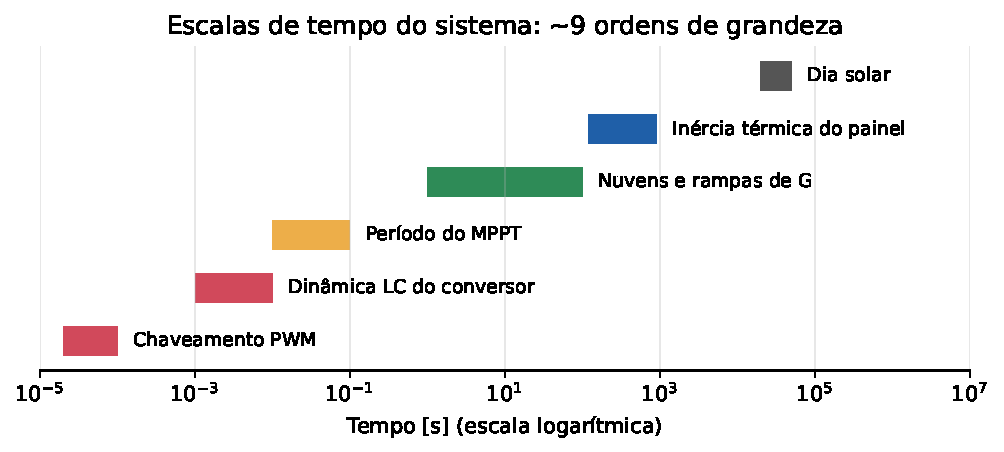
\includegraphics[width=0.85\linewidth]{figs/fig_escalas.pdf}
\caption{Escalas de tempo dos fenômenos do sistema.}
\label{fig:escalas}
\end{figure}

Um sistema com escalas tão separadas é chamado \textbf{rígido} (\emph{stiff}). Simular 12
horas com passo de microssegundos é inviável. A solução é usar uma \textbf{hierarquia de
modelos}, cada um com o nível de detalhe adequado ao que se quer observar:

\begin{center}\small
\begin{tabular}{lll}
\toprule
Modelo & Para quê & Duração simulada \\
\midrule
Chaveado & Validar o modelo médio, ver o \emph{ripple} & milissegundos \\
Médio & Transitórios do controle, perfil EN 50530 & segundos a minutos \\
Quase-estático & Dia inteiro & horas \\
\bottomrule
\end{tabular}
\end{center}

Cada simplificação será \emph{justificada}, comparando-a com o modelo mais detalhado no
intervalo em que ambos podem ser simulados.

% ================================================================ 3
\Needspace{12\baselineskip}
\section{Melhoria 1 -- Um painel virtual fiel}

\subsection{A física da célula solar}

Uma célula de silício é uma \textbf{junção P-N}: um ``sanduíche'' de duas camadas de silício
dopadas de forma diferente. Quando um fóton com energia suficiente é absorvido, ele cria
um par elétron-lacuna; o campo elétrico da junção separa esse par e gera uma corrente,
a \textbf{fotocorrente} $\Ipv$, proporcional à irradiância $G$.

Mas a junção também é um \textbf{diodo}. Quando a célula está polarizada (tem tensão nos
terminais), parte da corrente ``vaza'' de volta pela junção. Quanto maior a tensão, maior
esse vazamento, que cresce \emph{exponencialmente}. É por isso que a curva I-V tem um
``joelho'': até certa tensão quase toda a fotocorrente sai pelos terminais; depois, o
diodo ``engole'' rapidamente a corrente.

\subsection{Circuito equivalente: de 1 para 2 diodos}

O trabalho anterior usou o modelo de \textbf{um diodo} (Figura~\ref{fig:circuitos}, à
esquerda). Na junção real há dois mecanismos físicos distintos de corrente:

\begin{itemize}
\item \textbf{Difusão} de portadores nas regiões neutras: domina em tensões altas (perto de
$V_{oc}$); fator de idealidade $a_1\approx1$.
\item \textbf{Recombinação} na região de depleção, causada por defeitos do cristal: domina em
tensões baixas e pouca luz; fator de idealidade $a_2\approx2$.
\end{itemize}

O modelo de 1 diodo ``mistura'' os dois num diodo com fator intermediário. Funciona bem
perto de 1000\,W/m², mas erra em baixa irradiância, que é justamente o regime das manhãs,
dos fins de tarde e das sombras. O modelo de \textbf{dois diodos} (Figura~\ref{fig:circuitos},
à direita) representa cada mecanismo separadamente.

\begin{figure}[h]
\centering
\begin{circuitikz}[scale=0.82, transform shape]
\draw (0,0) to[I, l=$I_{pv}$] (0,3) -- (4,3);
\draw (1.6,3) to[D, l_=$D$] (1.6,0);
\draw (3.2,3) to[R, l_=$R_p$] (3.2,0);
\draw (3.2,3) to[R, l=$R_s$, i=$I$, -o] (6,3);
\draw (0,0) to[short, -o] (6,0);
\draw (6,3) to[open, v^>=$V$] (6,0);
\node at (3,-0.8) {\small modelo de 1 diodo};
\end{circuitikz}
\hspace{0.8cm}
\begin{circuitikz}[scale=0.82, transform shape]
\draw (0,0) to[I, l=$I_{pv}$] (0,3) -- (4.6,3);
\draw (1.4,3) to[D, l_=$D_1$] (1.4,0);
\draw (2.9,3) to[D, l_=$D_2$] (2.9,0);
\draw (4.4,3) to[R, l_=$R_p$] (4.4,0);
\draw (4.4,3) to[R, l=$R_s$, i=$I$, -o] (7.2,3);
\draw (0,0) to[short, -o] (7.2,0);
\draw (7.2,3) to[open, v^>=$V$] (7.2,0);
\node at (3.6,-0.8) {\small modelo de 2 diodos};
\end{circuitikz}
\caption{Circuitos equivalentes da célula. $R_s$ representa as perdas ôhmicas (contatos,
trilhas); $R_p$ representa correntes de fuga pelas bordas e defeitos.}
\label{fig:circuitos}
\end{figure}

\subsection{A equação do painel}

Aplicando a Lei de Kirchhoff das correntes no nó superior do circuito de 2 diodos:
\begin{equation}
I = \Ipv
 - I_{01}\left[\exp\!\left(\frac{V+R_sI}{a_1\Vt}\right)-1\right]
 - I_{02}\left[\exp\!\left(\frac{V+R_sI}{a_2\Vt}\right)-1\right]
 - \frac{V+R_sI}{R_p},
\qquad \Vt = \frac{N_s\,k\,T}{q}
\label{eq:2d}
\end{equation}
em que $N_s$ é o número de células em série, $k$ a constante de Boltzmann e $q$ a carga do
elétron. A dependência com o clima entra por:
\begin{align}
\Ipv(G,T) &= \frac{G}{G_n}\Big[I_{pv,n} + K_i\,(T-T_n)\Big] \label{eq:ipv}\\[4pt]
I_{0k}(T) &= I_{0k,n}\left(\frac{T}{T_n}\right)^{\gamma_k}
  \exp\!\left[\frac{q\,E_g}{a_k\,k}\left(\frac{1}{T_n}-\frac{1}{T}\right)\right],
  \qquad k=1,2 \label{eq:i0}
\end{align}
com $T_n=298{,}15$\,K (25\,°C), $E_g\approx1{,}12$\,eV (\emph{gap} do silício), $\gamma_1\approx3$
e $\gamma_2\approx3/2$. A Figura~\ref{fig:iv} mostra o formato típico das curvas resultantes.

\begin{figure}[h]
\centering
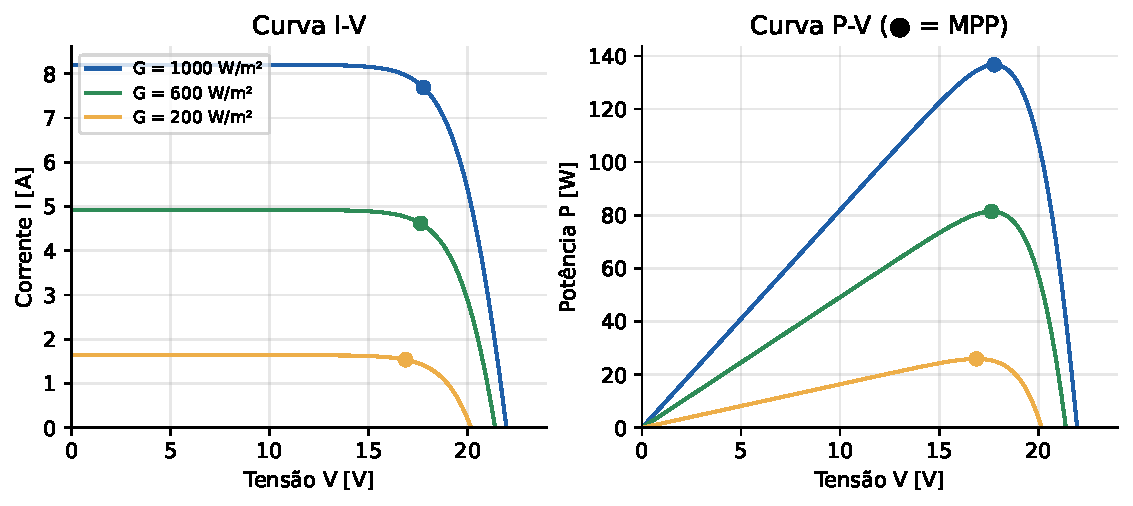
\includegraphics[width=0.95\linewidth]{figs/fig_iv_pv.pdf}
\caption{Curvas I-V e P-V típicas para três irradiâncias (ilustrativo). A irradiância
afeta principalmente a corrente; o MPP (pontos) se desloca.}
\label{fig:iv}
\end{figure}

\begin{atencao}[: um erro a corrigir]
O trabalho anterior usou $T_{ref}=278$\,K. O correto é $298$\,K (25\,°C, condição padrão de
teste). Esse detalhe desloca todas as curvas dependentes da temperatura.
\end{atencao}

\subsection{Extração dos parâmetros: por que o ajuste anterior falhou}

O fabricante não informa $R_s$, $R_p$, $I_{01}$, $I_{02}$; eles precisam ser
\emph{estimados} a partir do que o datasheet informa. O trabalho anterior tinha 3 incógnitas
e impôs essencialmente \textbf{uma} condição (passar pelo MPP). Com menos equações do que
incógnitas há infinitas soluções, e o algoritmo numérico parou em uma degenerada
($R_s\approx10^{-16}\,\Omega$, $I_s\approx10^{-20}$\,A). O problema era \textbf{mal posto};
a culpa não era do \texttt{fsolve}.

\begin{intuicao}[: o sistema mal posto]
É como tentar descobrir dois números sabendo apenas que a soma deles é 10. O computador
devolve \emph{um} par que satisfaz a condição, mas não há como saber se é o par certo.
\end{intuicao}

\paragraph{Formulação bem posta.} Fixamos os fatores de idealidade nos valores físicos
($a_1=1$, $a_2=2$). Restam cinco incógnitas,
$\boldsymbol\theta=[I_{pv,n},\,I_{01,n},\,I_{02,n},\,R_s,\,R_p]$, para as quais escrevemos
cinco condições tiradas do datasheet:
\begin{align}
&(1)\ \text{curto-circuito:} && I(V=0) = I_{sc}\\
&(2)\ \text{circuito aberto:} && I(V=V_{oc}) = 0\\
&(3)\ \text{ponto de máxima potência:} && I(V=V_{mp}) = I_{mp}\\
&(4)\ \text{o MPP é um máximo:} && \left.\frac{dP}{dV}\right|_{mp} = I_{mp}+V_{mp}\left.\frac{dI}{dV}\right|_{mp} = 0\\
&(5)\ \text{coeficiente térmico de } V_{oc}: && V_{oc}(T_n+\Delta T) - V_{oc,n} = K_v\,\Delta T
\end{align}

A condição (4) é a que faltou no trabalho anterior. A derivada $dI/dV$ sai por
\textbf{diferenciação implícita} da equação~\eqref{eq:2d}. Definindo
\begin{equation}
g_k = \frac{I_{0k}}{a_k\Vt}\exp\!\left(\frac{V+R_sI}{a_k\Vt}\right),
\qquad g = g_1+g_2+\frac{1}{R_p}
\quad\Longrightarrow\quad
\frac{dI}{dV} = -\frac{g}{1+R_s\,g}.
\label{eq:didv}
\end{equation}

O sistema é resolvido com \texttt{lsqnonlin} do MATLAB, com limites ($R_s>0$, $R_p>0$,
$I_0>0$) e variáveis escalonadas (pois $I_0\sim10^{-9}$ enquanto $R_p\sim10^{2}$). Os limites
tornam a solução degenerada impossível.

\subsection{Como calcular $I(V)$ a cada passo de simulação}

A equação~\eqref{eq:2d} tem $I$ dos dois lados e não possui solução explícita. Usamos o
\textbf{método de Newton-Raphson}: escrevendo $F(I)=0$, iteramos
\begin{equation}
I^{(m+1)} = I^{(m)} - \frac{F(I^{(m)})}{F'(I^{(m)})},
\qquad F'(I) = -1 - R_s\,g.
\end{equation}

\begin{intuicao}[: Newton-Raphson]
Para achar onde uma curva cruza o zero, o método traça a reta tangente no ponto atual e vê
onde \emph{ela} cruza o zero. Esse cruzamento vira o novo chute. Perto da solução, o número
de casas decimais corretas praticamente dobra a cada iteração.
\end{intuicao}

Como a corrente muda pouco entre dois passos de simulação, usamos a solução do passo anterior
como chute inicial (\emph{warm start}): bastam 2--3 iterações por passo.

\subsection{Validação}
\begin{itemize}
\item Digitalizar as curvas I-V do datasheet em várias irradiâncias e temperaturas.
\item Calcular o RMSE e o erro relativo de $P_{max}$ em cada condição.
\item Comparar 1 diodo $\times$ 2 diodos: espera-se que coincidam em 1000\,W/m² e que o
modelo de 2 diodos seja melhor em 200\,W/m².
\end{itemize}

\begin{resumo}
O painel é modelado por uma equação implícita com 5 parâmetros, extraídos de forma bem posta
a partir de 5 informações do datasheet, resolvida por Newton-Raphson e validada contra as
curvas do fabricante.
\end{resumo}

% ================================================================ 4
\Needspace{12\baselineskip}
\section{Melhoria 2 -- Sombreamento parcial e diodos de bypass}

\subsection{A física: células em série}

As células de um módulo estão ligadas \textbf{em série}, como as pilhas de uma lanterna.
Consequência: todas são atravessadas pela \emph{mesma corrente}. Se uma célula é sombreada,
sua fotocorrente cai. Se a corrente imposta pela fileira for maior do que a que essa célula
consegue gerar, ela é forçada à \textbf{polarização reversa}: passa a \emph{consumir} potência,
esquenta (\emph{hot spot}) e derruba a potência do módulo inteiro.

Para evitar isso, os módulos têm \textbf{diodos de bypass} ligados em antiparalelo com cada
grupo de células (\emph{submódulo}). Quando a tensão do grupo tenta ficar negativa, o diodo
conduz, ``desvia'' o excesso de corrente e limita a tensão do grupo a $\approx -V_F$
(cerca de $-0{,}4$\,V).

\begin{center}
\begin{circuitikz}[scale=0.8, transform shape]
\draw (0,0) to[I, l=$\text{sub.\,1}\ (G_1)$] (0,2.6);
\draw (2.2,0) to[D, l_=$D_{bp1}$] (2.2,2.6);
\draw (0,2.6) to[I, l=$\text{sub.\,2}\ (G_2)$] (0,5.2);
\draw (2.2,2.6) to[D, l_=$D_{bp2}$] (2.2,5.2);
\draw (0,0) -- (2.2,0);
\draw (0,2.6) -- (2.2,2.6);
\draw (0,5.2) -- (2.2,5.2);
\draw (2.2,5.2) to[short, -o] (4,5.2);
\draw (2.2,0) to[short, -o] (4,0);
\draw (4,5.2) to[open, v^>=$V_{pv}$] (4,0);
\draw[decorate, decoration={brace, amplitude=5pt}] (-3.3,0.1) -- node[left=6pt, font=\small]{$V_1$} (-3.3,2.5);
\draw[decorate, decoration={brace, amplitude=5pt}] (-3.3,2.7) -- node[left=6pt, font=\small]{$V_2$} (-3.3,5.1);
\end{circuitikz}\\[2pt]
{\small Dois submódulos em série, cada um com seu diodo de bypass: $V_{pv}=V_1+V_2$, mesma corrente $I$.}
\end{center}

\subsection{A matemática}

Dividimos o módulo em $N_{sub}$ submódulos, cada um com sua irradiância $G_j$ e sua tensão
$V_j$, todos com a mesma corrente $I$:
\begin{align}
I &= I_{cel,j}(V_j, G_j, T) + I_{bp}(V_j), \qquad j=1,\dots,N_{sub}\\
I_{bp}(V_j) &= I_{0,bp}\left[\exp\!\left(\frac{-V_j}{n_{bp}V_{t,bp}}\right)-1\right]\\
\vpv &= \sum_{j=1}^{N_{sub}} V_j
\end{align}
em que $I_{cel,j}$ é a equação~\eqref{eq:2d} aplicada ao submódulo $j$. O diodo de bypass é
modelado pela equação exponencial de Shockley (e não por um ``corte'' do tipo
$\max(V,-V_F)$), porque uma função suave evita descontinuidades que atrapalham o Newton.

\paragraph{Como resolver.} O conversor impõe $\vpv$; queremos $I$. As incógnitas algébricas
são $\mathbf z=[I,V_1,\dots,V_{N_{sub}}]$ e as equações são as $N_{sub}$ equações dos
submódulos mais a soma das tensões: $N_{sub}+1$ equações e $N_{sub}+1$ incógnitas. Resolve-se
por Newton multivariável com jacobiano analítico (esparso, pois cada equação só depende de
$I$ e de um $V_j$). Uma alternativa elegante é entregar todo o DAE ao \texttt{ode15s} com uma
\textbf{matriz de massa singular}: as linhas algébricas recebem zero na diagonal.

\subsection{Por que aparecem vários picos}

Considere três submódulos, um deles sombreado (350\,W/m²):
\begin{itemize}
\item \textbf{Corrente baixa} (menor que a corrente de curto do sombreado): os três geram.
A tensão é alta e a corrente é baixa $\to$ \textbf{um} pico de potência.
\item \textbf{Corrente alta}: o submódulo sombreado não consegue acompanhar, é ``bypassado''
e contribui com $\approx-V_F$. Só os outros dois geram; a tensão é menor e a corrente é
maior $\to$ \textbf{outro} pico.
\end{itemize}

A curva I-V ganha ``degraus'' e a curva P-V ganha \textbf{até $N_{sub}$ máximos locais}
(Figura~\ref{fig:sombra}). Qual deles é o global depende da intensidade da sombra.

\begin{figure}[h]
\centering
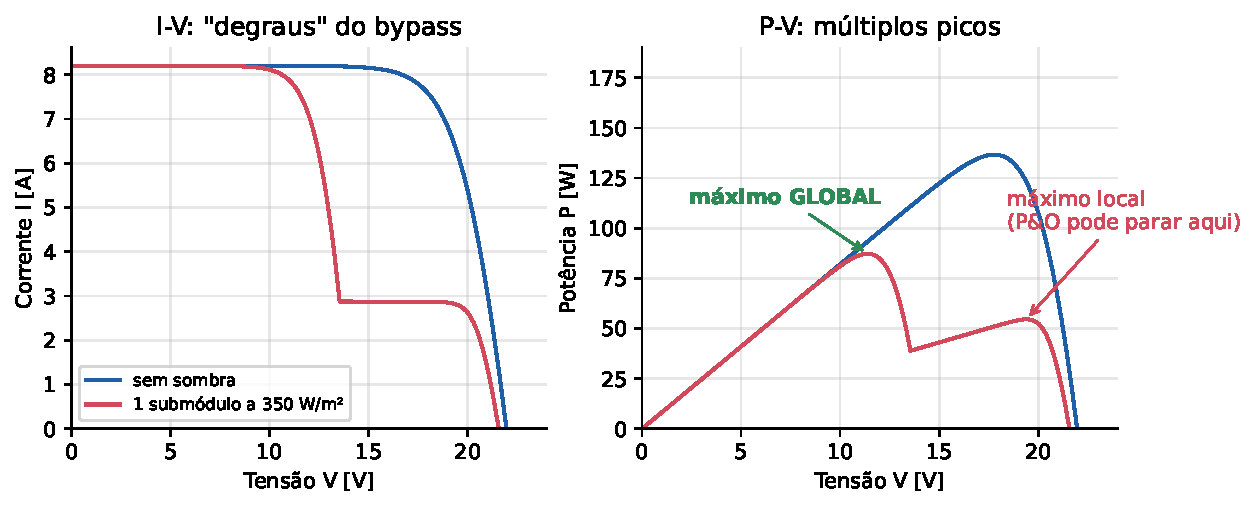
\includegraphics[width=0.95\linewidth]{figs/fig_sombra.pdf}
\caption{Efeito do sombreamento parcial (ilustrativo, 3 submódulos com bypass). Na curva
sombreada, o maior pico está em tensão \emph{baixa}; um algoritmo que parte da tensão alta
encontra primeiro o pico menor.}
\label{fig:sombra}
\end{figure}

\subsection{Validação}
\begin{itemize}
\item Com $G_1=G_2=\dots$, o resultado deve coincidir exatamente com o modelo do item 3.
\item Os picos devem cair próximos a múltiplos de $\approx0{,}8\,V_{oc,sub}$ (regra empírica
da literatura).
\item A potência dissipada no bypass deve ser $\approx V_F\,(I-I_{sc,\,\text{sombreado}})$.
\end{itemize}

\begin{atencao}[: limitação declarada]
Não será modelada a ruptura reversa das células (modelo de Bishop). Como o bypass entra em
condução muito antes da ruptura, a simplificação é aceitável e será mencionada no relatório.
\end{atencao}

% ================================================================ 5
\Needspace{12\baselineskip}
\section{Melhoria 3 -- O painel esquenta: modelo térmico}

\subsection{A física}

Um painel ao sol recebe muito mais energia do que converte em eletricidade (tipicamente
$\sim$15--20\,\%). O restante vira calor. Como a tensão de uma célula \emph{cai} com a
temperatura (cerca de $-0{,}3$ a $-0{,}4\,\%$/°C na potência), um painel quente produz menos.

O painel é tratado como um único corpo de temperatura uniforme (\textbf{capacitância térmica
concentrada}). A hipótese é razoável porque o módulo é fino e conduz calor internamente bem
mais rápido do que troca calor com o ar (número de Biot pequeno).

\subsection{O balanço de energia}

``Variação da energia armazenada = o que entra $-$ o que sai'':
\begin{equation}
m\,c_p\,\frac{dT}{dt} =
\underbrace{\alpha\,A\,G}_{\text{sol absorvido}}
-\underbrace{P_{el}}_{\text{vira eletricidade}}
-\underbrace{h_c\,A_t\,(T-T_{amb})}_{\text{convecção (vento)}}
-\underbrace{\varepsilon\,\sigma\,A_t\,(T^4-T_{\text{céu}}^4)}_{\text{radiação para o céu}}
\label{eq:termico}
\end{equation}
com $\alpha\approx0{,}9$ (absortância), $A$ a área do módulo e $A_t\approx2A$ (frente e verso).
Correlações usadas:
\begin{align}
h_c &\approx 5{,}7 + 3{,}8\,v_{vento}\quad[\mathrm{W/m^2K}] && \text{(convecção forçada, McAdams)}\\
T_{\text{céu}} &\approx 0{,}0552\,T_{amb}^{1{,}5}\quad[\mathrm K] && \text{(Swinbank)}
\end{align}

\begin{intuicao}[: o acoplamento]
O termo $P_{el}$ é o elo entre a parte elétrica e a térmica: a energia que o MPPT extrai
como eletricidade \emph{não} aquece o painel. Um MPPT melhor deixa o painel um pouco mais
frio, o que aumenta a tensão, o que aumenta a potência. É um laço de realimentação física.
\end{intuicao}

\subsection{Constante de tempo}

Linearizando a radiação ($h_{rad}\approx4\varepsilon\sigma T^3\approx6$\,W/m²K) e usando
uma capacidade térmica por área típica de $m c_p/A\approx11$\,kJ/(m²K):
\begin{equation}
\tau = \frac{m\,c_p}{(h_c+h_{rad})\,A_t}\approx\frac{11\,000}{(11+6)\cdot2}\approx 5\text{ min}.
\end{equation}

Ou seja, o painel funciona como um \textbf{filtro passa-baixas}: uma nuvem de poucos segundos
quase não altera sua temperatura (Figura~\ref{fig:termico}).

\begin{figure}[h]
\centering
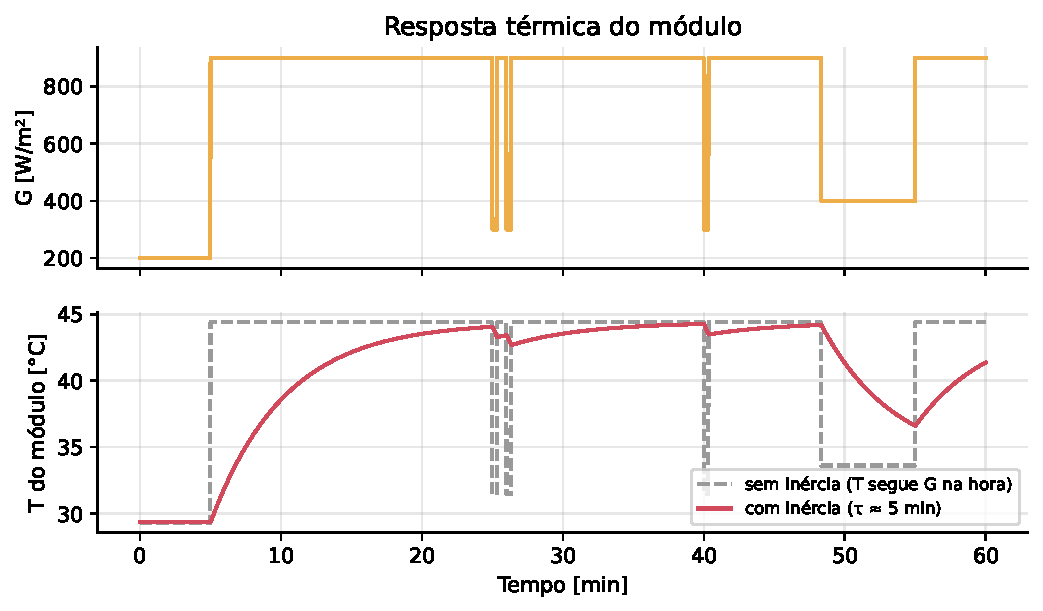
\includegraphics[width=0.85\linewidth]{figs/fig_termico.pdf}
\caption{Resposta térmica (ilustrativo). A curva tracejada mostra o que um modelo sem inércia
preveria; a contínua, o modelo dinâmico. Nuvens curtas são praticamente filtradas.}
\label{fig:termico}
\end{figure}

\subsection{Calibração e validação pelo NOCT}

O datasheet informa o \textbf{NOCT}: a temperatura da célula com $G=800$\,W/m²,
$T_{amb}=20$\,°C, vento de 1\,m/s e painel em circuito aberto ($P_{el}=0$). Em regime
permanente ($dT/dt=0$), a equação~\eqref{eq:termico} deve reproduzir $T=$\,NOCT nessas
condições. Se não reproduzir, ajusta-se $h_c$, o parâmetro mais incerto. Em seguida,
compara-se com a correlação padrão $T=T_{amb}+\frac{\mathrm{NOCT}-20}{800}\,G$.

% ================================================================ 6
\Needspace{12\baselineskip}
\section{Melhoria 4 -- Um conversor com perdas}

\subsection{Como o buck-boost funciona}

\begin{figure}[h]
\centering
\begin{circuitikz}[scale=0.9, transform shape]
\draw (0,0) to[I, l=$i_{pv}$] (0,3) -- (1.8,3);
\draw (1.8,3) to[C, l_=$C$, v^>=$v_{pv}$] (1.8,0);
\draw (1.8,3) to[spst, l=$S$] (4.2,3);
\draw (4.2,3) to[L, l_=$L$, i>^=$i_L$] (4.2,0);
\draw (6.8,3) to[D, l_=$D$] (4.2,3);
\draw (6.8,3) to[battery1, l_=$V_{bat}$] (6.8,0);
\draw (0,0) -- (6.8,0);
\node[font=\small] at (7.35,2.75) {$-$};
\node[font=\small] at (7.35,0.25) {$+$};
\end{circuitikz}
\caption{Conversor buck-boost (versão inversora). O painel e o capacitor $C$ estão na
entrada; a chave $S$ é comandada por PWM com razão cíclica $d$.}
\label{fig:buckboost}
\end{figure}

O conversor alterna entre duas configurações milhares de vezes por segundo:
\begin{itemize}
\item \textbf{Chave fechada} (fração $d$ do período): o painel ``carrega'' o indutor com energia.
\item \textbf{Chave aberta} (fração $1-d$): o indutor descarrega essa energia na bateria pelo diodo.
\end{itemize}
Ajustando $d$, ajusta-se quanta corrente é puxada do painel e, portanto, \emph{em que ponto
da curva I-V ele opera}. Em regime ideal, $V_{bat}/\vpv = d/(1-d)$: para $d<0{,}5$ abaixa a
tensão, para $d>0{,}5$ eleva.

\begin{atencao}[: inconsistência no trabalho anterior]
A equação (14) do trabalho anterior ($v_o=v_i\,D/(1-D)$) está correta; a equação (16), que
deveria ser a mesma relação, aparece invertida. Além disso, a frequência de chaveamento
usada (2\,kHz) é baixa para essa potência; será adotado $f_s\approx20$\,kHz, com $L$ e $C$
redimensionados por critério de \emph{ripple}.
\end{atencao}

\subsection{Onde a energia se perde}

\begin{center}\small
\begin{tabular}{lll}
\toprule
Elemento & Perda & Representação \\
\midrule
Indutor & resistência do cobre & $r_L$ em série \\
MOSFET & condução & $R_{on}$ quando fechado \\
Diodo & queda de tensão + resistência & $V_F + R_D$ quando conduz \\
Capacitor & resistência série equivalente & $r_C$ (\emph{ESR}) \\
Chaveamento & sobreposição de $V$ e $I$ nas transições & $P_{sw}=\tfrac12 V_{sw}I_L(t_r+t_f)f_s$ \\
\bottomrule
\end{tabular}
\end{center}

\subsection{Modelo chaveado}

Com $q(t)\in\{0,1\}$ indicando o estado da chave (gerado comparando $d$ com uma portadora
dente-de-serra), as Leis de Kirchhoff dão:
\begin{align}
q=1:\quad & L\frac{di_L}{dt} = \vpv - i_L(r_L+R_{on}), &
            & C\frac{d\vpv}{dt} = \ipv - i_L\\
q=0:\quad & L\frac{di_L}{dt} = -(V_{bat}+V_F) - i_L(r_L+R_D), &
            & C\frac{d\vpv}{dt} = \ipv
\end{align}

\subsection{Modelo médio}

Se o chaveamento é muito mais rápido que a dinâmica de interesse, podemos substituir as
grandezas por suas \textbf{médias em um período de chaveamento}. Isso equivale a trocar
$q(t)$ por $d(t)$:
\begin{align}
L\frac{di_L}{dt} &= d\,\vpv - (1-d)(V_{bat}+V_F) - i_L\big[r_L + d\,R_{on} + (1-d)R_D\big] \label{eq:medio1}\\
C\frac{d\vpv}{dt} &= \ipv(\vpv) - d\,i_L \label{eq:medio2}
\end{align}

No equilíbrio (derivadas nulas), obtêm-se $i_L=\ipv/d$, o ganho estático com perdas (que
deixa de ser exatamente $d/(1-d)$) e a eficiência
$\eta_{conv}=(1-d)\,i_L\,V_{bat}/(\vpv\,\ipv)$.

\begin{intuicao}[: modelo médio]
É como olhar um ventilador girando: você não enxerga cada pá, só um disco borrado. O modelo
médio ``enxerga o disco'': perde o detalhe do liga-desliga, mas descreve bem o movimento
lento e é centenas de vezes mais rápido de simular.
\end{intuicao}

\subsection{Quando a média vale -- e o perigo do DCM}

O modelo médio exige duas condições:
\begin{enumerate}
\item \textbf{Separação de frequências:} $f_s \gg f_0 = \dfrac{D}{2\pi\sqrt{LC}}$.
\item \textbf{Ripple pequeno e condução contínua (CCM):} a corrente no indutor nunca chega a
zero, isto é, $i_{L,\text{médio}} > \Delta i_L/2$, com $\Delta i_L = \dfrac{\vpv\,d}{L\,f_s}$.
\end{enumerate}

\begin{atencao}[: modo descontínuo]
Em baixa irradiância (manhã, fim de tarde, sombra forte) a corrente cai e o conversor pode
entrar em \textbf{DCM} (\emph{Discontinuous Conduction Mode}). Nesse regime as
equações~\eqref{eq:medio1}--\eqref{eq:medio2} deixam de valer. O modelo deve detectar essa
situação e tratá-la, um ponto raramente explorado em trabalhos de graduação.
\end{atencao}

\subsection{Validação: chaveado $\times$ médio}

A Figura~\ref{fig:chav} mostra a comparação que será feita: o modelo chaveado (com
\emph{ripple}) e o médio devem coincidir na média. Também será verificado o
\textbf{balanço de energia}: $P_{in}-P_{out}-\sum\text{perdas}\approx0$, um teste simples e
poderoso de que o código está correto.

\begin{figure}[h]
\centering
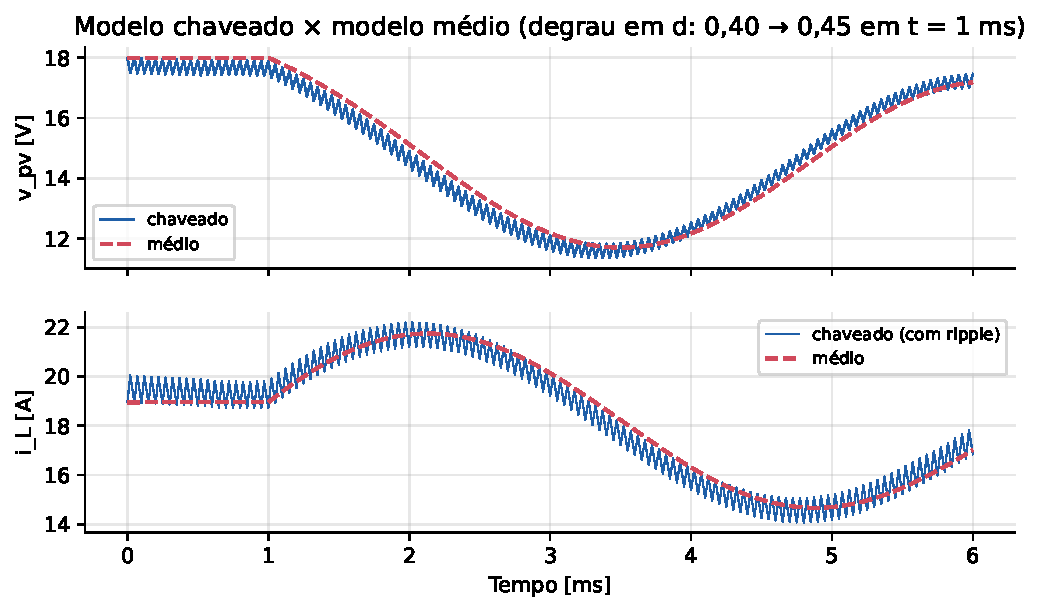
\includegraphics[width=0.85\linewidth]{figs/fig_chaveado_medio.pdf}
\caption{Modelo chaveado $\times$ modelo médio (ilustrativo, sem perdas) após um degrau na
razão cíclica. O médio acompanha a média do chaveado e dispensa simular cada comutação.}
\label{fig:chav}
\end{figure}

% ================================================================ 7
\Needspace{12\baselineskip}
\section{Projeto do controle: linearização}

\subsection{A malha de controle}

O controle tem duas camadas:
\begin{center}
\begin{tikzpicture}[node distance=1.1cm,
  bloco/.style={draw,rounded corners,minimum height=0.9cm,align=center,thick,font=\small},
  seta/.style={-{Stealth[length=2.5mm]},thick}]
\node[bloco,fill=azul!5] (m) {MPPT\\\footnotesize(lento, externo)};
\node[bloco,fill=azul!12,right=of m] (p) {PI de tensão\\\footnotesize(rápido, interno)};
\node[bloco,fill=amarelo!25,right=of p] (c) {Conversor\\+ painel};
\draw[seta] (m) -- node[above,font=\footnotesize]{$V_{ref}$} (p);
\draw[seta] (p) -- node[above,font=\footnotesize]{$d$} (c);
\draw[seta] (c.south) -- ++(0,-0.5) -| node[pos=0.25,below,font=\footnotesize]{$\vpv$} (p.south);
\end{tikzpicture}
\end{center}
O MPPT decide \emph{qual} tensão o painel deve ter; o PI faz o painel \emph{ir até} essa
tensão manipulando $d$. A malha interna precisa ser bem mais rápida que a externa.

\subsection{Linearização do painel}

Em torno de um ponto de operação $(V_0,I_0)$, o painel se comporta como uma
\textbf{resistência dinâmica}: $\tilde\imath_{pv}\approx-\tilde v_{pv}/r_{pv}$, com
$r_{pv}=-\,dV/dI|_0$. No MPP vale um resultado elegante: como $dP/dV=0$, temos
$dI/dV=-I/V$, logo
\begin{equation}
r_{pv}\big|_{MPP} = \frac{V_{mp}}{I_{mp}}.
\end{equation}
À esquerda do MPP o painel parece uma fonte de corrente ($r_{pv}$ grande); à direita, uma
fonte de tensão ($r_{pv}$ pequeno). \textbf{A planta muda com o ponto de operação.}

\subsection{Função de transferência}

Perturbando o modelo médio (sem perdas, para clareza) com $x=X+\tilde x$ e $d=D+\tilde d$,
desprezando produtos de perturbações e aplicando a transformada de Laplace:
\begin{equation}
G_{vd}(s)=\frac{\tilde v_{pv}(s)}{\tilde d(s)}
=-\,\frac{L\,I_L\,s + D\,(V_{pv}+V_{bat})}{L\,C\,s^2 + \dfrac{L}{r_{pv}}\,s + D^2},
\qquad
\omega_0=\frac{D}{\sqrt{LC}},\quad
\zeta=\frac{1}{2\,D\,r_{pv}}\sqrt{\frac{L}{C}}.
\end{equation}

Três leituras importantes:
\begin{itemize}
\item O \textbf{sinal negativo} é físico: aumentar $d$ puxa mais corrente do painel e a
tensão cai. O controlador precisa ter o sinal invertido.
\item É um sistema de \textbf{2ª ordem subamortecido}, o que explica o \emph{overshoot}
observado (e não explicado) no trabalho anterior.
\item O amortecimento $\zeta$ \textbf{depende de $r_{pv}$}, isto é, do ponto de operação
(Figura~\ref{fig:bode}).
\end{itemize}

\begin{figure}[h]
\centering
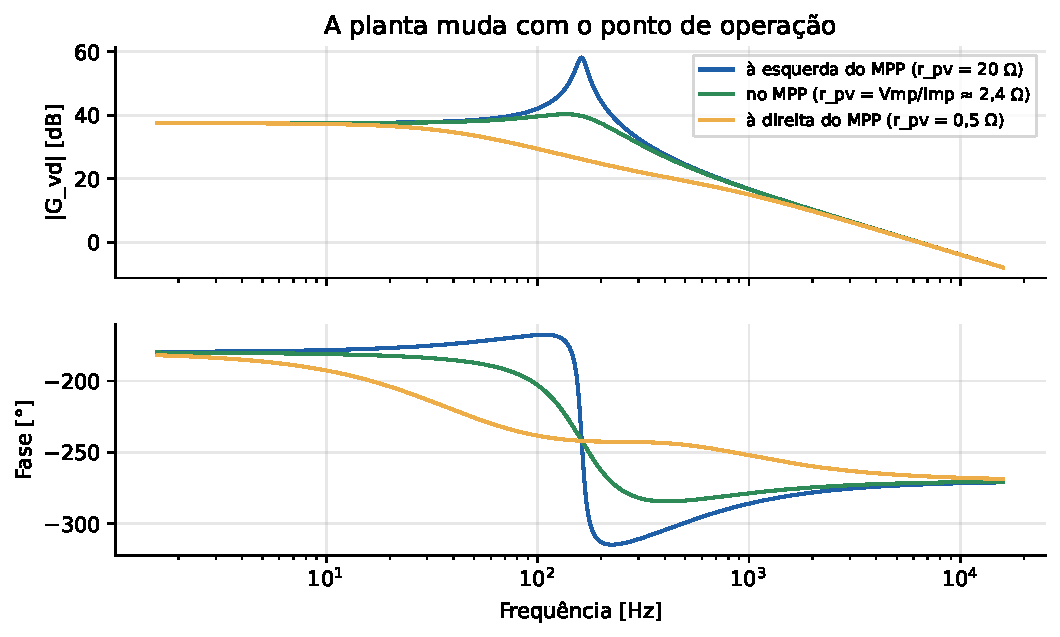
\includegraphics[width=0.85\linewidth]{figs/fig_bode.pdf}
\caption{Diagrama de Bode de $G_{vd}(s)$ em três pontos de operação (ilustrativo). À esquerda
do MPP a ressonância é pouco amortecida; o PI precisa ser estável em todos os casos.}
\label{fig:bode}
\end{figure}

\subsection{Projeto do PI}

O controlador $C(s)=K_p\left(1+\frac{1}{T_i\,s}\right)$ será projetado para:
frequência de cruzamento abaixo da ressonância e bem abaixo de $f_s$; margem de fase de
45--60°; atraso do PWM modelado por $e^{-sT_s/2}$ (aproximação de Padé). Ferramentas:
\texttt{bode}, \texttt{margin}, \texttt{pidtune}. A robustez será verificada traçando as
margens para vários pontos de operação.

\paragraph{Validação.} Um degrau \emph{pequeno} em $d$ aplicado ao modelo não linear deve
reproduzir a resposta de $G_{vd}(s)$. Um degrau \emph{grande} mostrará onde a linearização
deixa de valer.

% ================================================================ 8
\Needspace{12\baselineskip}
\section{Melhoria 5 -- Três algoritmos de MPPT}

Para uma comparação justa, os três algoritmos atuam sobre a mesma referência $V_{ref}$, com
a mesma malha PI e o mesmo período de amostragem $T_a$.

\subsection{P\&O -- Perturba e Observa}

\begin{intuicao}[: o andarilho de olhos vendados]
Alguém tenta chegar ao topo de um morro de olhos vendados. Dá um passo; se subiu, continua
na mesma direção; se desceu, vira para o outro lado. Funciona muito bem com um morro só.
\end{intuicao}

\begin{equation}
\Delta P\cdot\Delta V > 0 \ \Rightarrow\ V_{ref} \mathrel{+}= \delta, \qquad
\Delta P\cdot\Delta V < 0 \ \Rightarrow\ V_{ref} \mathrel{-}= \delta.
\end{equation}

\paragraph{Escolha dos parâmetros (critério de Femia).}
\begin{itemize}
\item \textbf{Período $T_a$:} deve ser maior que o tempo de acomodação da malha de tensão.
Se o MPPT medir antes do transitório acabar, confunde a dinâmica do conversor com uma
mudança de potência.
\item \textbf{Passo $\delta$:} em regime, o P\&O oscila em três níveis em torno do MPP. Pela
aproximação parabólica $P\approx P_{mp}-\tfrac12|P''|(V-V_{mp})^2$, a perda por oscilação é
proporcional a $\delta^2$. Passo grande rastreia rápido, mas oscila muito.
\item \textbf{Deriva por rampa:} se $G$ sobe durante $T_a$, o $\Delta P$ medido mistura o efeito
do passo com o efeito do sol, e o algoritmo pode andar para o lado errado. As rampas da norma
EN 50530 testam exatamente isso.
\end{itemize}

\subsection{InC -- Condutância Incremental}

Parte da condição exata de máximo:
\begin{equation}
\frac{dP}{dV}=I+V\frac{dI}{dV}=0 \quad\Longleftrightarrow\quad \frac{dI}{dV}=-\frac{I}{V}.
\end{equation}
Comparando a condutância incremental medida $\Delta I/\Delta V$ com a condutância instantânea
$-I/V$: se forem iguais (dentro de uma tolerância $\varepsilon$), \textbf{mantém} $V_{ref}$;
se $\Delta I/\Delta V>-I/V$, o ponto está à esquerda do MPP e $V_{ref}$ aumenta; caso
contrário, diminui. O caso $\Delta V=0$ é tratado pelo sinal de $\Delta I$.

\begin{intuicao}[: o andarilho com nível de bolha]
O andarilho agora mede a inclinação do chão. Quando ela é zero, ele sabe que está no topo
e \emph{para}, em vez de ficar oscilando. Mas continua enxergando só o chão sob os pés:
também pode parar no topo do morro menor.
\end{intuicao}

\subsection{PSO -- Enxame de Partículas}

\begin{intuicao}[: o bando de pássaros]
Um bando procura comida espalhado pelo campo. Cada pássaro lembra o melhor lugar que já
visitou e ouve os outros gritarem onde está o melhor lugar de todos. A cada voo, mistura
três tendências: continuar onde estava indo, voltar para o seu melhor lugar e ir para o
melhor lugar do bando. Por explorar o campo todo, o bando acha o \emph{maior} morro.
\end{intuicao}

Cada partícula $i$ é uma tensão candidata $x_i$. A atualização é:
\begin{align}
v_i &\leftarrow \underbrace{w\,v_i}_{\text{inércia}}
  + \underbrace{c_1 r_1\,(p_{best,i}-x_i)}_{\text{memória própria}}
  + \underbrace{c_2 r_2\,(g_{best}-x_i)}_{\text{memória do enxame}}\\
x_i &\leftarrow x_i + v_i
\end{align}
com $r_1,r_2\sim\mathcal U(0,1)$ e valores típicos $N=4$--5 partículas, $w\approx0{,}4$,
$c_1\approx1{,}2$, $c_2\approx2$.

\paragraph{Detalhes de implementação.}
\begin{itemize}
\item Só existe \emph{um} painel: as partículas são avaliadas \textbf{uma de cada vez}
(aplica $V_{ref}=x_i$, espera $T_a$, mede $P$). Uma iteração custa $N\cdot T_a$.
\item \textbf{Inicialização:} partículas espalhadas em $[0{,}1\,V_{oc};\,0{,}9\,V_{oc}]$, de
preferência perto dos múltiplos de $\approx0{,}8\,V_{oc,sub}$ onde os picos tendem a ficar.
\item \textbf{Convergência:} quando as partículas se agrupam (dispersão abaixo de uma
tolerância), fixa-se $V_{ref}=g_{best}$: oscilação zero em regime.
\item \textbf{Reinicialização:} se $|\Delta P/P|$ ultrapassar um limiar (ex.\ 10\,\%), as
condições mudaram e o enxame é espalhado de novo.
\end{itemize}

\begin{resumo}[: o dilema central]
Durante a exploração, o PSO passa de propósito por pontos ruins e perde energia. Ele
compensa se o ganho de achar o pico global for maior que essa perda, o que depende de
quanto tempo a sombra dura e de quão frequente ela é. A simulação vai \emph{quantificar}
esse dilema.
\end{resumo}

\begin{table}[h]
\centering\small
\begin{tabular}{llll}
\toprule
Método & Informação usada & Ponto forte & Ponto fraco \\
\midrule
P\&O & variação de potência & simples, barato & oscila; cai em máximo local \\
InC & derivada $dI/dV$ & para no MPP; menos oscilação & cai em máximo local \\
PSO & varredura global & encontra o máximo global & exploração custa energia e tempo \\
\bottomrule
\end{tabular}
\caption{Comparação qualitativa esperada dos três algoritmos.}
\end{table}

% ================================================================ 9
\Needspace{12\baselineskip}
\section{Testes e métricas}

\subsection{A métrica principal: eficiência de rastreamento}

\begin{equation}
\eta_{MPPT} = \frac{\displaystyle\int P_{pv}(t)\,dt}{\displaystyle\int P_{mpp,\,global}(t)\,dt}
\end{equation}

$P_{mpp,global}(t)$ é o \textbf{oráculo}: o máximo global da curva P-V nas condições daquele
instante, calculado offline por varredura densa do modelo estático.

\begin{atencao}[: por que ``global'']
Se o denominador usasse o máximo \emph{local}, o P\&O pareceria 99\,\% eficiente mesmo
preso no pico errado. Comparar contra o máximo global é o que revela a perda por sombreamento.
\end{atencao}

Métricas complementares: energia diária (Wh), tempo de convergência após uma perturbação,
amplitude da oscilação em regime, eficiência do conversor $\eta_{conv}$ e eficiência total
$\eta_{MPPT}\cdot\eta_{conv}$.

\subsection{Teste 1 -- Perfil dinâmico da norma EN 50530}

A norma europeia EN~50530 define sequências de \textbf{rampas de irradiância} (de níveis
baixos a médios e de médios a altos, com inclinações das mais lentas às muito rápidas,
intercaladas com patamares) para avaliar o desempenho dinâmico de MPPTs. A tabela exata de
rampas será extraída da norma ou da literatura que a reproduz. Como o teste dura minutos, ele
é simulado com o \textbf{modelo médio} e o controle completo. É onde as diferenças entre P\&O
e InC sob rampa devem aparecer.

\subsection{Teste 2 -- Um dia real em Florianópolis}

\begin{itemize}
\item \textbf{Dados:} irradiância, temperatura ambiente e vento de um dia de Florianópolis,
obtidos do PVGIS (Comissão Europeia) ou de estação do INMET.
\item \textbf{Eventos sintéticos documentados:} dados horários não têm transitórios rápidos;
por isso são adicionadas passagens de nuvens e um evento de \textbf{sombra parcial} (por
exemplo, a sombra de um poste atravessando os submódulos entre 14\,h e 15\,h). O relatório
deixará claro: \emph{dados climáticos reais + cenários de sombra projetados}.
\item \textbf{Simulação multi-taxa:} 12 horas com passos de microssegundos é inviável. Usa-se o
modelo \textbf{quase-estático}: como o conversor e o PI acomodam muito mais rápido que $T_a$,
a cada passo do MPPT considera-se o conversor em equilíbrio, e o MPPT vira um mapa discreto
$V_{ref}[k]\mapsto P(V_{ref}[k],G,T)$. O modelo térmico é integrado com passo de segundos.
\item \textbf{Justificativa da simplificação:} em um trecho de alguns minutos, simula-se também
o modelo médio completo e mostra-se que os dois produzem a mesma energia.
\end{itemize}

% ================================================================ 10
\Needspace{12\baselineskip}
\section{Plano de trabalho}

\begin{table}[h]
\centering\small
\renewcommand{\arraystretch}{1.2}
\begin{tabularx}{\linewidth}{c >{\bfseries}l X}
\toprule
Etapa & Bloco & Entregável \\
\midrule
1 & Painel & Extração de parâmetros (2 diodos), validação contra o datasheet, comparação com 1 diodo \\
2 & Sombreamento & Modelo com bypass; curvas com múltiplos picos; validação no caso uniforme \\
3 & Conversor & Modelo médio com perdas; modelo chaveado; comparação; balanço de energia; verificação de DCM \\
4 & Controle & Linearização, $G_{vd}(s)$, projeto do PI e análise de robustez \\
5 & MPPT & P\&O, InC e PSO com o mesmo $T_a$ e a mesma malha interna \\
6 & Térmico & Modelo térmico calibrado pelo NOCT e acoplado à parte elétrica \\
7 & Resultados & EN 50530 + dia em Florianópolis; tabela comparativa; conclusão quantitativa \\
\bottomrule
\end{tabularx}
\caption{Sequência de implementação. A etapa 1 é a fundação: sem um painel validado, nenhum
resultado posterior é confiável.}
\end{table}

\subsection*{Pendências antes de começar}
\begin{enumerate}
\item \textbf{Datasheet do ZTROON ZTP-160M}: número de células, quantidade de diodos de
bypass, $I_{sc}$, $V_{oc}$, $I_{mp}$, $V_{mp}$, $K_i$, $K_v$, NOCT e curvas I-V. O trabalho
anterior traz dados inconsistentes ($P_{max}=4{,}8$\,W e 11 células no texto, mas
$\approx121$\,W na simulação), então é preciso conferir na fonte.
\item \textbf{MATLAB com toolboxes}: Optimization (\texttt{lsqnonlin}) e Control System
(\texttt{bode}, \texttt{margin}, \texttt{pidtune}).
\end{enumerate}

\begin{resumo}[: o que torna esta proposta diferente]
\begin{itemize}
\item Mantém o mesmo painel e a mesma ferramenta, usando o trabalho anterior como linha de base.
\item Cada melhoria corrige uma simplificação anterior e \emph{mede} o impacto dela.
\item Cada modelo é validado contra uma referência (datasheet, NOCT, modelo chaveado, linearização).
\item A conclusão passa de ``funciona'' para ``funciona $X\,\%$, nesta condição, por este motivo''.
\end{itemize}
\end{resumo}

% ================================================================ REF
\begin{thebibliography}{99}\small
\bibitem{barbi} BARBI, I. \emph{Modelagem de conversores CC-CC empregando modelo médio em
espaço de estados}. Florianópolis: Edição do Autor, 2015.
\bibitem{erickson} ERICKSON, R. W.; MAKSIMOVIĆ, D. \emph{Fundamentals of Power Electronics}.
2.\ ed. Springer, 2001.
\bibitem{villalva} VILLALVA, M. G.; GAZOLI, J. R.; RUPPERT FILHO, E. Comprehensive approach to
modeling and simulation of photovoltaic arrays. \emph{IEEE Transactions on Power Electronics},
v.\ 24, n.\ 5, p.\ 1198--1208, 2009.
\bibitem{ishaque} ISHAQUE, K.; SALAM, Z.; TAHERI, H. Simple, fast and accurate two-diode
model for photovoltaic modules. \emph{Solar Energy Materials and Solar Cells}, v.\ 95, n.\ 2,
p.\ 586--594, 2011.
\bibitem{femia} FEMIA, N.; PETRONE, G.; SPAGNUOLO, G.; VITELLI, M. Optimization of perturb
and observe maximum power point tracking method. \emph{IEEE Transactions on Power Electronics},
v.\ 20, n.\ 4, p.\ 963--973, 2005.
\bibitem{hussein} HUSSEIN, K. H.; MUTA, I.; HOSHINO, T.; OSAKADA, M. Maximum photovoltaic
power tracking: an algorithm for rapidly changing atmospheric conditions. \emph{IEE
Proceedings -- Generation, Transmission and Distribution}, v.\ 142, n.\ 1, p.\ 59--64, 1995.
\bibitem{ishaquepso} ISHAQUE, K.; SALAM, Z. A deterministic particle swarm optimization
maximum power point tracker for photovoltaic system under partial shading condition.
\emph{IEEE Transactions on Industrial Electronics}, v.\ 60, n.\ 8, p.\ 3195--3206, 2013.
\bibitem{duffie} DUFFIE, J. A.; BECKMAN, W. A. \emph{Solar Engineering of Thermal Processes}.
4.\ ed. Wiley, 2013.
\bibitem{en50530} CENELEC. \emph{EN 50530: Overall efficiency of grid connected photovoltaic
inverters}. Bruxelas, 2010.
\bibitem{pinho} PINHO, J. T.; GALDINO, M. A. \emph{Manual de Engenharia para Sistemas
Fotovoltaicos}. Rio de Janeiro: CEPEL/CRESESB, 2014.
\bibitem{anterior} DAGA, A.; SCHNEIDER JUNIOR, M. \emph{Energia Fotovoltaica com Conversor
Buck-Boost}. Trabalho final de DAS5109, UFSC.
\end{thebibliography}

\end{document}
